\documentclass[aspectratio=169]{beamer}
\usetheme{default}
\usepackage{amsmath,amssymb,tikz}
\usetikzlibrary{arrows.meta}
\setbeamertemplate{navigation symbols}{}
\title{Shortest Paths: Dijkstra's Algorithm}
\subtitle{Algorithms and Data Structures -- Week 9}
\date{}
\begin{document}

\frame{\titlepage}

\begin{frame}{The single-source shortest-path problem}
\begin{itemize}
  \item Directed graph $G=(V,E)$, edge weights $w(u,v) \ge 0$, source $s$
  \item Find $\delta(s,v)$, the length of a shortest path from $s$ to every $v$
  \item Applications: road navigation, network routing (OSPF), game AI
\end{itemize}
\end{frame}

\begin{frame}{Example graph}
\centering
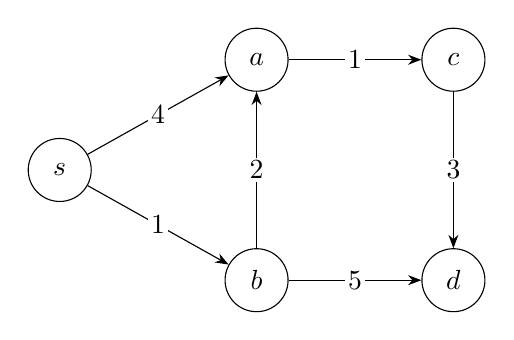
\begin{tikzpicture}[>=Stealth, node distance=2.2cm, every node/.style={circle,draw,minimum size=8mm}]
  \node (s) at (0,0) {$s$};
  \node (a) at (2.5,1.4) {$a$};
  \node (b) at (2.5,-1.4) {$b$};
  \node (c) at (5,1.4) {$c$};
  \node (d) at (5,-1.4) {$d$};
  \begin{scope}[every node/.style={fill=white,inner sep=1pt}]
  \draw[->] (s) -- node {4} (a);
  \draw[->] (s) -- node {1} (b);
  \draw[->] (b) -- node {2} (a);
  \draw[->] (a) -- node {1} (c);
  \draw[->] (b) -- node {5} (d);
  \draw[->] (c) -- node {3} (d);
  \end{scope}
\end{tikzpicture}
\end{frame}

\begin{frame}{Relaxation}
\begin{itemize}
  \item Keep an estimate $d[v] \ge \delta(s,v)$, initially $d[s]=0$, $d[v]=\infty$
  \item Relax edge $(u,v)$: \quad if $d[u]+w(u,v) < d[v]$ then $d[v] \gets d[u]+w(u,v)$, $\pi[v]\gets u$
  \item Predecessors $\pi$ form the shortest-path tree
\end{itemize}
\end{frame}

\begin{frame}{The algorithm}
\begin{enumerate}
  \item Put all vertices in a min-priority queue $Q$ keyed by $d[\cdot]$
  \item While $Q$ is not empty: $u \gets$ \textsc{Extract-Min}$(Q)$
  \item For each edge $(u,v)$: relax, and \textsc{Decrease-Key} $v$ if $d[v]$ changed
\end{enumerate}
\medskip
Greedy: the vertex with the smallest tentative distance is final.
\end{frame}

\begin{frame}{Trace on the example}
\centering
\begin{tabular}{c|ccccc}
step & $s$ & $a$ & $b$ & $c$ & $d$\\ \hline
init & 0 & $\infty$ & $\infty$ & $\infty$ & $\infty$\\
extract $s$ & \textbf{0} & 4 & 1 & $\infty$ & $\infty$\\
extract $b$ & & 3 & \textbf{1} & $\infty$ & 6\\
extract $a$ & & \textbf{3} & & 4 & 6\\
extract $c$ & & & & \textbf{4} & 6\\
extract $d$ & & & & & \textbf{6}
\end{tabular}
\end{frame}

\begin{frame}{Why it is correct}
\begin{itemize}
  \item Invariant: when $u$ is extracted, $d[u] = \delta(s,u)$
  \item Proof idea: a shorter path would leave the set of finished vertices through some edge $(x,y)$;
        with $w \ge 0$ we get $d[y] \le d[u]$, contradicting the choice of $u$
  \item Fails with negative edges $\Rightarrow$ use Bellman--Ford
\end{itemize}
\end{frame}

\begin{frame}{Running time}
\centering
\begin{tabular}{l|l}
priority queue & time \\ \hline
array & $O(V^2)$ \\
binary heap & $O((V+E)\log V)$ \\
Fibonacci heap & $O(E + V \log V)$
\end{tabular}
\medskip

Dense graphs: the array is fine. Sparse graphs: use a heap.
\end{frame}

\end{document}
